% $Id: INF_Diplomarbeit.tex 1660 2010-02-25 13:57:42Z tkren $
%
% TU Wien - Faculty of Informatics
% thesis template
%
% This template is using the memoir document class, see
% <http://www.ctan.org/tex-archive/macros/latex/contrib/memoir/memman.pdf>
% <http://www.ctan.org/info/latex-samples/MemoirChapStyles/MemoirChapStyles.pdf>
%
% For questions and comments send an email to
% Thomas Krennwallner <tkren@kr.tuwien.ac.at>
%

								
\documentclass[a4paper,12pt, oneside]{memoir}
%\chapterstyle{veelo}
\usepackage{graphicx} 
\usepackage{placeins}
\usepackage{caption}


\chapterstyle{madsen}
\setlength{\parskip}{6pt plus 1pt minus 1pt}
\setlength{\parindent}{0pt}

\usepackage{TUINFDA}

\thesistitle{Cluster visualization for interactive maps}
\thesisdate{\the\day.\the\month.\the\year}

\thesisdegree{Diplom-Ingenieur}
\thesiscurriculum{Software Engineering and Internet Computing}
\thesisverfassung{Verfasser}
\thesisauthor{Josef Dabernig}
\thesismatrikelno{0927232}
% \thesisauthoraddress{} % your address

\thesisbetreuung{Betreuer}
\thesisbetreins{Prof.~Dr.~A Min Tjoa}
\thesisbetrzwei{Univ.-Ass.~Dr. Amin Anjomshoaa}

\newcommand{\EnableCustomThesisLayout}{
\setheaderspaces{*}{1.5cm}{*}
}

\usepackage{multirow}
\usepackage{rotating}

\begin{document}


% the front matter                                                 
\frontmatter

% $Id: titlepage.tex 2165 2010-08-07 04:42:52Z tkren $
%
% TU Wien - Faculty of Informatics
% thesis titlepage
%
% This titlepage is using the geometry package, see
% <http://www.ctan.org/macros/latex/contrib/geometry/geometry.pdf>
%
% For questions and comments send an email to
% Thomas Krennwallner <tkren@kr.tuwien.ac.at>
%

% setup page dimensions for titlepage
\newgeometry{left=2.4cm,right=2.4cm,bottom=2.5cm,top=2cm}

% force baselineskip and parindent
\newlength{\tmpbaselineskip}
\setlength{\tmpbaselineskip}{\baselineskip}
\setlength{\baselineskip}{13.6pt}
\newlength{\tmpparindent}
\setlength{\tmpparindent}{\parindent}
\setlength{\parindent}{17pt}
\newlength{\tmpparskip}
\setlength{\tmpparskip}{\parskip}
\setlength{\parskip}{0pt}


% first titlepage
\thispagestyle{tuinftitlepage}

%
% Kludge: for each titlepage set \pagenumbering to a different
% style. This is used to fix a problem with hyperref, because there
% are multiple "page 1" and hyperref hates that
%
\pagenumbering{Alph}

\begin{center}
%
\begin{minipage}[t][5.2cm][b]{\linewidth}%
    \centering%
    %\renewcommand{\baselinestretch}{0.9} % very long titles need to tweak baselinestretch...
    \thesistitlefontHUGE\sffamily\bfseries\tuinfthesistitle%
\end{minipage}


\vspace{1.3cm}

{\thesistitlefontLARGE\sffamily \tuinfthesistype}

\vspace{6mm}

% {\thesistitlefontlarge\sffamily zur Erlangung des akademischen Grades}

\vspace{6mm}

% {\thesistitlefontLARGE\sffamily\bfseries \tuinfthesisdegree}

\vspace{6mm}

% {\thesistitlefontlarge\sffamily im Rahmen des Studiums}

\vspace{6mm}

% {\thesistitlefontLarge\sffamily\bfseries \tuinfthesiscurriculum}

\vspace{6.5mm}

% {\thesistitlefontlarge\sffamily eingereicht von}

\vspace{6mm}

{\thesistitlefontLarge\sffamily\bfseries \tuinfthesisauthor}

\vspace{1.5mm}

{\thesistitlefontlarge\sffamily Matrikelnummer \tuinfthesismatrikelno} 

\vspace{1.5cm}

\begin{minipage}[t][1.7cm][t]{\textwidth}%
  \vspace{0pt}\raggedright\thesistitlefontnormalsize\sffamily
  %
  an der

  Fakult\"{a}t f\"{u}r Informatik der Technischen Universit\"{a}t Wien
\end{minipage}

\begin{minipage}[t][4cm][t]{\textwidth}%
  \vspace{0pt}\sffamily\thesistitlefontnormalsize\raggedright
  %
  Betreuung

  \tuinfthesisbetreuung: \tuinfthesisbetreins

%  \raggedright Mitwirkung: \tuinfthesisbetrzwei

\end{minipage}

% we want a german date, then switch back to english
 \selectlanguage{ngerman}
 \begin{minipage}[t][2cm][t]{\textwidth}%
  \vspace{0pt}\sffamily\thesistitlefontnormalsize
  \begin{tabbing}%
    Wien, \tuinfthesisdate
    %    \> \begin{minipage}[t][0.5cm][t]{51mm}\centering (Unterschrift \tuinfthesisverfassung)\end{minipage}
%    \> \begin{minipage}[t][0.5cm][t]{51mm}\centering (Unterschrift \tuinfthesisbetreuung)\end{minipage}
    \end{tabbing}
\end{minipage}
\selectlanguage{english}

\end{center}

% we want an empty page right after first titlepage
\cleardoublepage

% we're done with the titlepages, proceed with default pagenumbering
\pagenumbering{roman}

% restore baselineskip
\setlength{\baselineskip}{\tmpbaselineskip}
\setlength{\parindent}{\tmpparindent}
\setlength{\parskip}{\tmpparskip}


% back to normal geometry
\restoregeometry


%%% Local Variables:
%%% TeX-PDF-mode: t
%%% TeX-debug-bad-boxes: t
%%% TeX-parse-self: t
%%% TeX-auto-save: t
%%% reftex-plug-into-AUCTeX: t
%%% End:

\EnableCustomThesisLayout
% \chapter*{Erklärung zur Verfassung der Arbeit}

\tuinfthesisauthor\\
% \tuinfthesisauthoraddress

\vspace*{1.2cm}

Hiermit erkläre ich, dass ich diese Arbeit selbständig verfasst habe, 
dass ich die verwendeten Quellen und Hilfsmittel vollständig angegeben 
habe und dass ich die Stellen der Arbeit - einschließlich Tabellen, 
Karten und Abbildungen -, die anderen Werken oder dem Internet im 
Wortlaut oder dem Sinn nach entnommen sind, auf jeden Fall unter Angabe 
der Quelle als Entlehnung kenntlich gemacht habe.\\



  \begin{tabbing}%
    \hspace{15mm} \= \hspace{65mm} \= \hspace{42mm} \kill
    \> Wien, \tuinfthesisdate \> {\raggedright\rule{51mm}{0.5pt}} \\
    \> \> \begin{minipage}[t][0.5cm][t]{51mm}\centering
 (Unterschrift \tuinfthesisverfassung)\end{minipage}
  \end{tabbing}


%
% abstract
%


\chapter*{Abstract}

This thesis investigates ways of visualization for presenting clustered information on maps. Performance and readability of digital mapping applications decreases when displaying large amounts of data. Clustering can be used to group overlapping items and reduce visual clutter of the map presentation. 

Visualization techniques for putting clusters on a map are researched and evaluated in an exploratory analysis. Existing concepts from visual cluster analysis and geovisualization, as well as established classifications form the foundations of the presented study. \textit{Map types} as well as \textit{cluster visualization techniques} are presented. The \textit{evaluation} classifies the stated techniques for cluster visualization on maps.

The presented map types for visualizing clusters range from standard, \textit{geographic maps} with markers, \textit{Heat maps} to \textit{Dot Grid maps} and a \textit{Voronoi} map. Cluster visualization techniques include \textit{icon-based/glyphs}, \textit{pixel-based}, as well as \textit{geometric/diagrams}. The evaluation of visualization techniques for clusters on a map proposes a custom set of criteria. \textit{Showing the number of items within clusters} is considered as a main feature of simple cluster visualizations on maps. Further, the study identifies \textit{showing cluster areas} and \textit{extra cluster information} as two additional aspects of primary interest when comparing approaches to cluster visualization on maps.   

The results are discussed and put into practice by evaluating the visual aspects of \textit{Geocluster}, a server-side clustering implementation for maps.
\newpage

\setcounter{tocdepth}{3}
\tableofcontents
\newpage

%TODO enable
%\listoffigures
\newpage

%\listoftables
\newpage

%
% start of the thesis
%
\mainmatter
\setcounter{secnumdepth}{3}


%
% intro
%

\chapter{Introduction}

Digital mapping applications on the Internet are strongly emerging. Big players like Google Maps\footnote{\url{https://maps.google.at}} and OpenStreetMap\footnote{\url{http://www.openstreetmap.org/ }} provide online maps, that users can view and interact with. Maps allow telling stories and communicating data in a visual way. They can be used to get a quick overview of points-of-interest in a certain area. If a large amount of information is contained in such an area, visual clutter is causing problems. Obviously, when telling a story, information needs to be told in a compact way as the human brain can only process a limited amount of data at the same time~\cite{noellenburg11geovis, Delort10vis}.

Clustering\footnote{\url{http://en.wikipedia.org/wiki/Cluster_analysis}} is a technique for grouping objects with similarities that can be used to reduce visual clutter as described before. Clustering points on a map enhances performance and readability of data-heavy map applications. Client-side clustering uses JavaScript to group overlapping items. Server-side clustering is needed when too many items slow down processing and create network bottle necks. This paper aims at discussing visual aspects of Geocluster, a server-side clustering implementation for maps. It considers well-separated, spatial clusters based on Euclidean distance.

The primary goal is to evaluate cluster visualization techniques for creating interactive maps based on large data sets. Visual ways for presenting clustered data on maps should be researched and summarized. Combining existing concepts from visual cluster analysis and geovisualization should provide a better understanding of theoretic backgrounds and put into context. The idea is to draw practical conclusions from the overlap of these two complex areas of research. Given the lack of existing publication on visualizing clusters on maps for reference, the study rather aim at exploration of concepts and ideas than being a complete reference. 


\section{Structure}

The given introduction is expanded by a discussion of \textit{related work} in the field of geovisualization and visual cluster analysis. In addition, the \textit{methods} being used to achieve the goal evaluating cluster visualization techniques for interactive maps.

Chapter \ref{chapter:foundations} describes the theoretic \textit{foundations} being researched. Basic concepts of geovisualization as visual variables, visual data exploration techniques and clutter reduction are explained.

Chapter \ref{chapter:results} discusses the main \textit{results} of the study. Map visualization types, as well as cluster visualization techniques are explained and summarized within an exploratory evaluation.

Chapter \ref{chapter:discussion} is a \textit{discussion} of the previously presented results and applies the evaluation of cluster visualization techniques for maps to the practical use case of Geocluster.

Chapter \ref{chapter:conclusion} finalizes the paper by drawing \textit{conclusions} of the presented results and discussion.


\section{Related work}

While many publications have been found on either cluster analysis or geovisualization, few of them touch upon both subjects at the same time. There hasn't been found any study that compares the different techniques for visualizing clusters on maps as its primary goal.

A primary resource instead are publications on individual approaches for cluster geovisualization: 
Heat maps \cite{geotree, hotmap}, Voronoi Diagrams \cite{Delort10vis, voromap}, Convex Hulls \cite{Cristani08geoimagemaps}. A well research blog article talks about different ways to visualize clusters on maps~\cite{web:clustering-google}. A more complex visualization is provided by Bristle Maps \cite{bristle}. Various cluster visualization techniques on maps are combined in \cite{andrienko2012sca}. Self-organizing maps represent clustered information in virtual space \cite{som}.

On a practical note, Leaflet.markercluster\footnote{\url{https://github.com/Leaflet/Leaflet.markercluster}}, the OpenLayers Cluster Strategy\footnote{\url{http://openlayers.org/dev/examples/strategy-cluster.html}} and MarkerClusterer for Google Maps\footnote{\url{http://google-maps-utility-library-v3.googlecode.com/svn/trunk/markerclusterer/docs/reference.html}} are common implementations for client-side clustering that visualize clusters on maps.

For classification of the researched techniques, 3 taxonomies have been considered. ``Visual variables'' by Jacques Bertin \cite{bertin67graphics, bertin83graphics} with some adjustments by Alan M. MacEachren \cite{MacEachren95maps} and Leland Wilkinson \cite{Wilkinson05grammar}. ``Classification of visual data exploration techniques'' by Daniel A. Keim~\cite{keim2001vis} and the ``Clutter Reduction Taxonomy'' by Geoffrey Ellis and Alan Dix~\cite{ellis08clutter}. Further, related taxonomies are found \cite{lohse, shneiderman}.
 
In addition, publications on cluster and multi-variate data visualization techniques \cite{ward02glyphs, zhang07thesis, ElmqvistDGHF08, hiervis}, geovisualization \cite{noellenburg11geovis, maceachren-geovis, MacEachren07cartovis} and diagrams \cite{ladenhauf12dia} are extensive resources for the individual topics being discussed in this paper.



\section{Method}

Scientific publications as well as real-world implementations have been researched in order to get a good overview of existing technologies related to visualizing clusters on maps. Given the lack of comparative publications in that particular field, papers on the individual topics of visualization, geovisualization and cluster analysis have been compared for overlapping concepts. As no fixed criteria, despite the general context and goals of the paper have been set, the research was mainly conducted in an explorative way. The criteria of published classifications and taxonomies have been reviewed to match the use case for visualizing clusters on web maps.

Based on an overview of foundations in geovisualization and cluster analysis, the main part of the study tries to enumerate the diverse approaches for visualizing clusters on maps. This is done from two perspectives: \textit{map visualization types} cover the whole visualization and \textit{cluster visualization techniques} focus on individual clusters being represented on maps. Finally, an attempt for classification has been made as part of evaluation based on exploratory analysis: custom criteria derived from existing taxonomies are defined and the researched technologies get classified amongst those criteria.









%
% foundations - vis
%

\chapter{Foundations}
\label{chapter:foundations-vis}

In the following chapter, foundations for visualizing clusters on a map will be discussed. Basics of geographic visualization and their driving forces lead to abstraction and clustering as a tool for simplifying information on maps. Visual variables, as well as classification approaches for geovisualization will be reviewed in order to discuss existing concepts for displaying aggregated data on a map.

Visualization is driven by the basic belief that `seeing' is a good way of understanding and generating knowledge. Humans have a very well developed sense of sight, a fact which is underlined by more of 50 percent of the neurons in our brain being used for vision.~\cite{vislecture}. 

MacEachren \& Kraak~\cite{maceachren-geovis} define that ``Geovisualization integrates approaches from visualization in scientific computing (ViSC), cartography, image analysis, information visualization, exploratory data analysis (EDA), and geographic information systems (GISystems) to provide theory, methods, and tools for visual exploration, analysis, synthesis, and presentation of geospatial data (any data having geospatial referencing).'' In his lecture notes on ``Geographic visualization'', Martin N\"{o}llenburg adds that more human-centered definitions exist and observes that the user's needs have to be taken into account for effective geovisualization techniques~\cite{noellenburg11geovis}.


The \textbf{goals of geovisualization} can be summarized using the \textit{map use cube} by MacEachren and Kraak \cite{MacEachren07cartovis}, which is illustrated in figure \ref{fig:geovis-cube}. The goals \textit{exploration, analysis, synthesis and presentation} are classified amongst three dimensions:

\begin{itemize}

\item The type of \textit{task} varies from \textit{knowledge construction} to \textit{information sharing}. While the first is about revealing unknowns and constructing new knowledge, the latter will primarily share existing knowledge.

\item The amount of \textit{interaction} ranges from \textit{high} to \textit{low}. A low level of interaction means a rather passive consumption of knowledge, instead a high level will allow the user to actively influence the visualization.

\item The \textit{users} of visualization are classified between \textit{public} and \textit{private} audiences. A single, private user with specialized skills might require different visualization techniques than large, public audiences.

\end{itemize}

In the given model of the map use cube, the goals of exploring, analyzing, synthesizing and presenting shift between the extremes of the three defined aspects. The first goal of exploring is classified as a task of knowledge construction, based on high interaction and targeted at a rather private audience. On the other hand, presenting is a task of information sharing that requires a low amount of interaction but is suitable for public audiences~\cite{noellenburg11geovis}.  

\begin{figure}[h]
  \begin{center}
    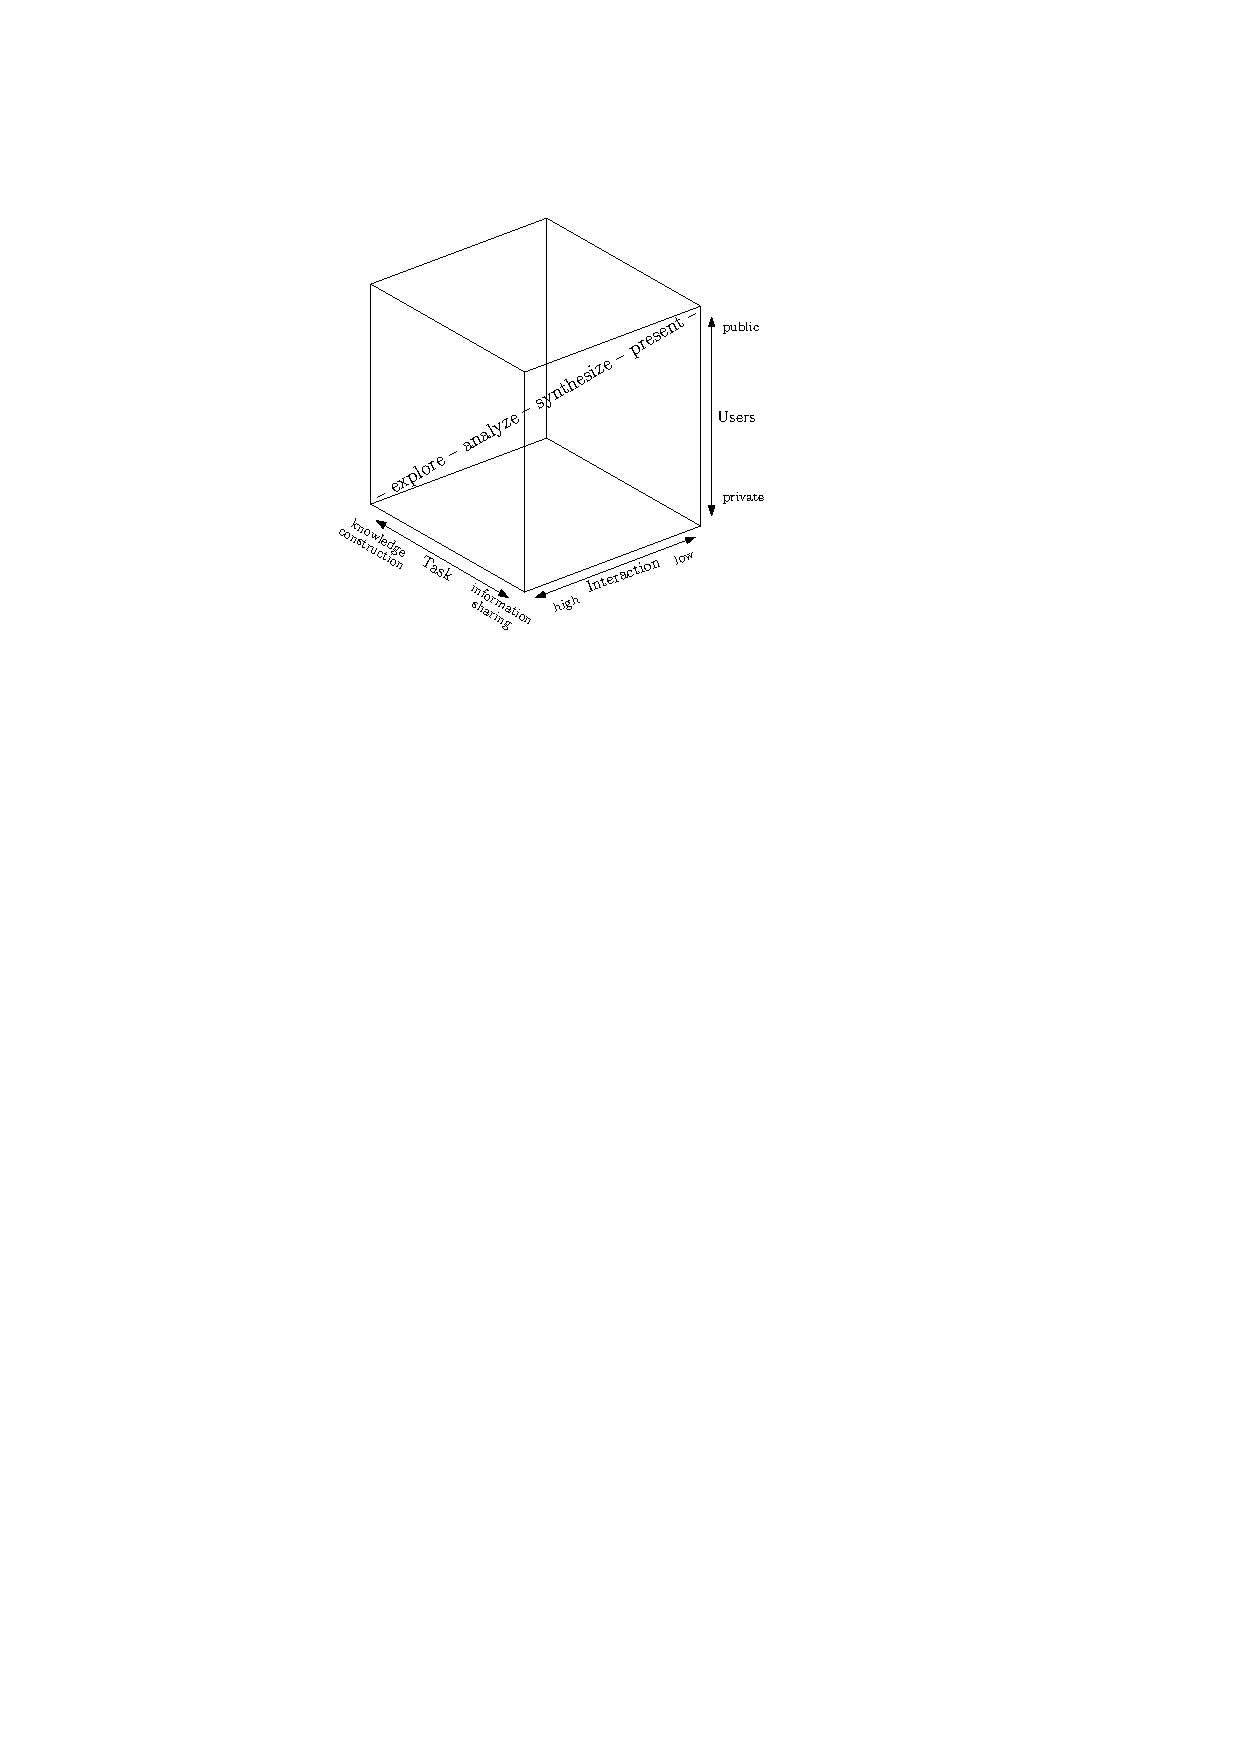
\includegraphics[width=0.65\textwidth]{figures/geovis_goals.pdf}
    \caption{The map use cube after MacEachren and Kraak \cite{MacEachren07cartovis} characterizing geovisualization goals in a three-dimensional space by their level of interaction, their audience, and the addressed tasks.~\cite{noellenburg11geovis}.}
    \label{fig:geovis-cube}
  \end{center}
\end{figure}


Cognitive aspects of visualization help us understand, how visual thinking works. Complex input is abstracted on the retina of the human eye and matched against a vast collection of patterns from experience. Despite generating realistic images, visualization can help generate new ideas by using abstraction to communicate patterns. The idea is to allow the user to join insight, draw conclusions and interact with the data by presenting it in a visual form that reduces the cognitive work needed to perform a given task~\cite{MACEACHREN90apattern, keim2001vis, noellenburg11geovis}. 

Various scientific publications~\cite{phillips82clutter, MACEACHREN90apattern, keim2001vis, harvey2008primer, ellis08clutter, Delort10vis, noellenburg11geovis} that have been researched for this thesis mention the importance of using abstraction for efficiently visualizing information. Especially maps can only highlight interesting information by filtering out unnecessary details of the environment. For example, a road map is better visualized on a clear background instead of satellite images that would distract the user from the primary goal of finding directions. The challenge is to balance realism and abstraction in geovisualization depending on the problem~\cite{noellenburg11geovis}.

\newpage
\section{Visual variables}
\label{chapter:vis-variables}

\begin{figure}[h]
  \begin{center}
    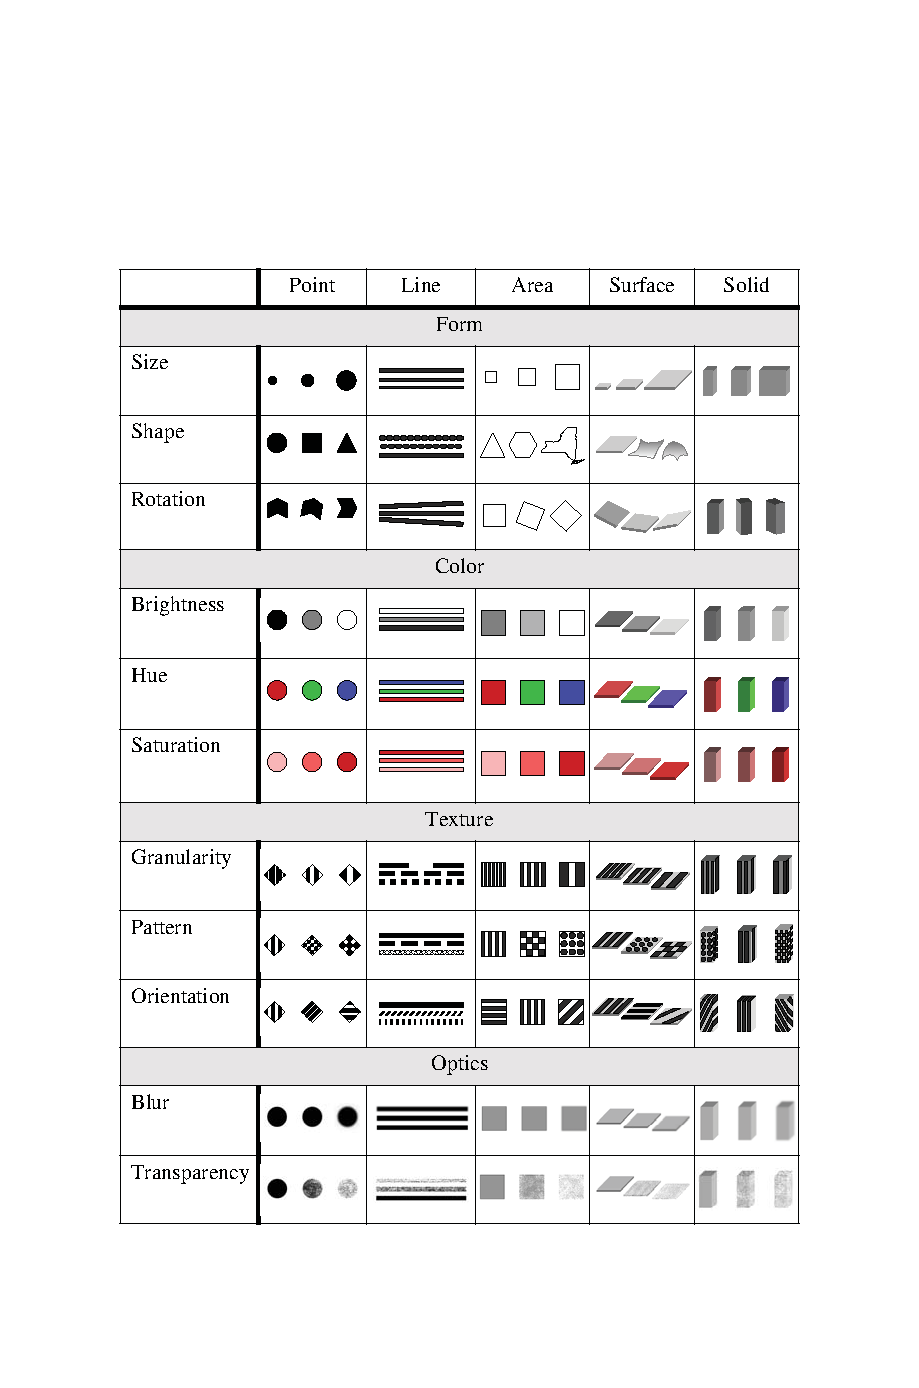
\includegraphics[width=0.8\textwidth]{figures/aesthetic_attributes.pdf}
    \caption{Aesthetic Attributes by Geometry~\cite{Wilkinson05grammar}.}
    \label{fig:aesthetic-attributes}
  \end{center}
\end{figure}

Information on a map is represented by symbols, point, lines or areas with properties such as color and shape. Bertin~\cite{bertin67graphics, bertin83graphics} has described the fundamental graphic variables for map and graphic design. While being written for hand-drawn maps on paper, the concepts described by Bertin are still applied in todays digital mapping applications and have been further developed by MacEachren~\cite{MacEachren95maps}.

The main variables, introduced by Bertin are: \textit{location}, \textit{size}, \textit{value}, \textit{texture}, \textit{color}, \textit{orientation} and \textit{shape}. MacEachren adds \textit{crispness}, \textit{resolution}, \textit{transparency} and \textit{arrangement} to the list and splits up color into its values of \textit{brightness}, \textit{saturation} and \textit{hue}. Figure \ref{fig:aesthetic-attributes} describes a similar list of aesthetic attributes by different geometries and groups the variables regarding \textit{form}, \textit{color}, \textit{texture} and \textit{optics}~\cite{Wilkinson05grammar}.

Each variable has a different potential for visualizing data of categorical information (nominal and ordinal) or numerical information (including intervals and ratios). For example, the size of a point can be used to describe a numeric ratio and different shapes may be used to distinguish items based on categories. On the other hand, different texture patterns only offer a limited set of possibilities and size shouldn't be used for describing nominal properties~\cite{noellenburg11geovis, MacEachren95maps}. 

\section{Visual data exploration techniques}
\label{vis-data-techniques}

Depending on the task and the type of data to be shown, different forms of visualization and techniques for exploring the data exist. Daniel A. Keim~\cite{keim2001vis} classifies such techniques using three criteria as depicted in figure \ref{fig:visual-techniques}: the \textit{data type} to be visualized, the \textit{technique} itself and the \textit{interaction and distortion} method~\cite{Delort10vis}:

\begin{itemize}

\item The \textbf{data type} is classified into \textit{one-dimensional} (as for example temporal data), \textit{two-dimensional} (geographical maps), \textit{multi-dimensional} (relational tables), \textit{text and hypertext} (articles and web documents), \textit{hierarchies and graphs} (networks) as well as \textit{algorithms and software} (such as debugging operations).

\item The \textbf{visualization techniques} are classified into \textit{standard 2d/3d displays} (x-y plots and landscapes), \textit{geometrically-transformed displays} (parallel coordinates), \textit{iconic displays} (glyphs), \textit{dense pixel displays} (recursive pattern) and \textit{stacked displays} (tree maps).

\item Finally, the third dimension describes the \textbf{interaction technique} being used, such as \textit{dynamic projection}, \textit{interactive filtering}, \textit{zooming}, \textit{distortion} and finally \textit{link \& brush} approaches.

\end{itemize}

\begin{figure}[h]
  \begin{center}
    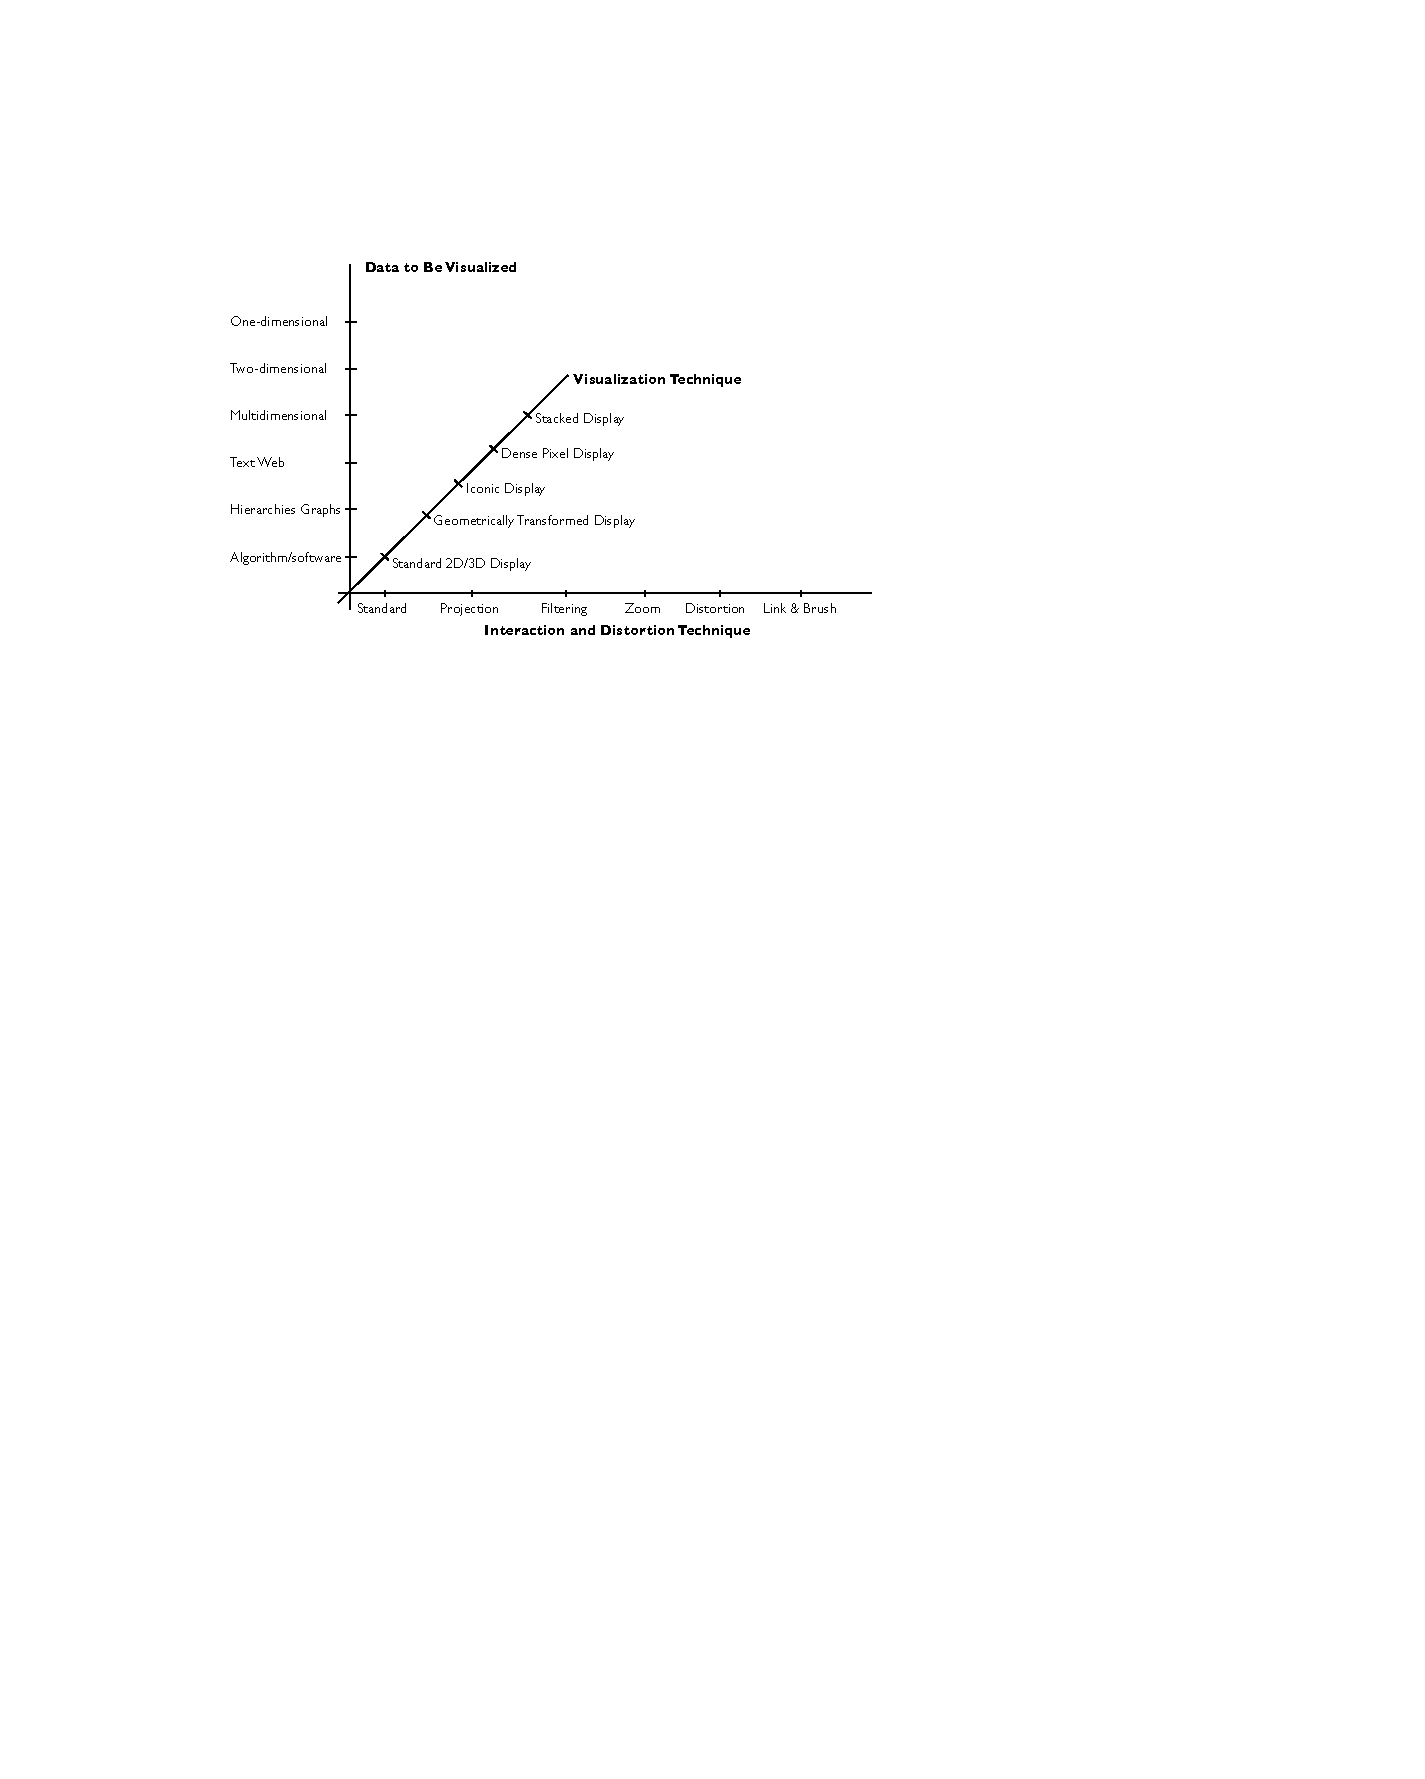
\includegraphics[width=1\textwidth]{figures/classes_visual_techniques.pdf}
    \caption{Classification of visual data exploration techniques based on~\cite{keim2001vis}.}
    \label{fig:visual-techniques}
  \end{center}
\end{figure}


With regards to visualizing clusters on a map, it appears that the visualization technique may be considered from two different view points:

\begin{itemize}

\item the visualization of the \textit{entire map} with clustered points on it, as well as

\item the visualization of an \textit{individual cluster}, placed on the map.

\end{itemize}

A typical map for representing spatially clustered data is based on a least \textit{two-dimensional data}, containing latitude and longitude information of cluster items. The map is presented in planar space, which classifies it amongst \textit{standard 2d/3d displays}. Common interaction techniques for maps are \textit{zooming} and \textit{panning} which allow the user to explore the 2-dimensional space and reveal details.

The visualization of individual clusters on the map is likely to be classified amongst \textit{iconic displays}. During the clustering process, individual points get aggregated, which potentially leads to multivariate aggregate information of item properties. Depending on the level of detail that clusters should expose, more complex visualization techniques may be possible. 

Approaches for visualization techniques of the entire map and individual clusters will be discussed further in chapter  \ref{state-vis}.

\section{Clutter reduction}
\label{clutter-reduction}

Clutter reduction is a way to enhance readability and general performance of maps. An early publication about \textit{visual clutter} on maps by Richard J. Phillips and Liza Noyes~\cite{phillips82clutter} states that ``reducing visual clutter improves map reading performance''. Clutter reduces the background visibility and prevents the user from understanding structure and content of the data being presented. This especially becomes true for visualizing large data sets on maps, so that properties of the data items are hardly visible~\cite{harvey2008primer, Delort10vis}.

Clustering of course is the approach for clutter reduction that is primarily being investigated for this thesis. In order to review the effectiveness and limitations of clustering, as well as the relationship that it has to other techniques in that field, it is helpful to review the ``Clutter Reduction Taxonomy'' by Geoffrey Ellis and Alan Dix~\cite{ellis08clutter}. It distinguishes between three main types of clutter reduction techniques:

\begin{itemize}

\item \textbf{appearance}: alter the look of data items by using techniques like \textit{sampling}, \textit{filtering}, \textit{changing point sizes}, \textit{changing opacity} or \textit{clustering}.

\item \textbf{spatial distortion}: displace the data items in ways as \textit{point/line displacement}, \textit{topological distortion}, \textit{space-filling}, \textit{pixel-plotting} or \textit{dimensional reordering}.

\item \textbf{temporal}: use \textit{animation} to reveal additional information.

\end{itemize}

In a next step, the stated techniques have been evaluated against a list of 8 high-level criteria~\cite{ellis08clutter}. For this thesis, the relevant information for the clustering technique have been extracted and will be outlined by each criterium:

\begin{enumerate}

\item \textit{avoids overlap}
\\ The major benefit is to reduce clutter, provide the ability of seeing and identifying patterns, have less hidden data, as well as giving more display space to points. Clustering can be used in such a way to avoid \textit{overplotting} by representing groups of points as single points.

\item \textit{keeps spatial information}
\\ Maintaining the correct coordinates of items is relevant, but the study also states that relative positions of points might have greater influence on orientation than just their exact coordinates. Clustering by definition looses the spatial information of individual points, but using aggregate values, like the centroid a cluster, as the position can be used for compensation. 

\item \textit{can be localized}
\\ The term localization is used to specify, if the display can be reduced to a specific region. This is usually provided by \textit{focus and context} techniques that reveal information underneath by zooming into an area. The study doesn't make a clear decision regarding the applicability of localization for clustering and states that different properties for spatial and non-spatial clustering apply. In the case of spatial clustering, localization is definitely possible and has been implemented, see chapter \ref{chapter:realization}.  

\item \textit{is scalable}
\\ Scalability of the clutter reduction technique with regards to large amounts of data is the goal of this criterium. The study admits that the meaning of large datasets is vaguely quantified. As one of the main goals for this thesis is to enhance performance for large data sets by using clustering, the technique is expected to satisfy this condition. Of course, the range of scalability depends on the implemented clustering algorithm. Also refer to the time complexity definitions in chapter \ref{clustering-algorithms}. 

\item \textit{is adjustable}
\\ If the user is able to control aspects of the visual display and adjust parameters of the system that influence the degree of display clutter. Scientific methods in cluster analysis tend to offer a a higher level of interactivity, while public facing clustering applications limit the amount of interactivity to controlling cluster sizes and the previously discussed localizing feature. 

\item \textit{can show point/line attribute}
\\ The goal is to map attributes of the data to properties like color, shape or opacity of the displayed points or lines. For clustering, this feature can be used in order to display aggregates of the multivariate data results from the clustering process. Further information can be found in chapter \ref{chapter:cluster-vis}.

\item \textit{can discriminate points/lines}
\\ Being to able to identify individual data items within a crowded display is the goal of this criterium. The study states the capability of clustering for detecting outliers as well as creating groups of points in order to satisfy this criterion. On the other hand, this classification appears unclear, as the grouping process of clustering aggregates individual information by definition and only makes it accessible by request or localization. 

\item \textit{can see overlap density}
\\ This helps to gauge the amount of overplotting, see where higher density regions are and understand the distribution of data underlying the visualization. Clustering can show the amount of items within clusters by using visual indicators as point size, opacity and color.  

\end{enumerate}



%
% state of the art
%

\chapter{State of the Art}
\label{chapter:state}


%
% objectives
%

\chapter{Further aspects}
\label{chapter:further-aspects}








%
% realization
%

\chapter{Conclusions}
\label{chapter:conclusions}



\section{Usability}
\label{chapter:objective-usability}

Clustering data on maps not only affects performance, it also changes the way, the user will see and interact with the clustered data. Ideally, the clustering process should support the user in the task of exploring a large data set on the map by compacting the amount of information that is visualized. The way, how the clustered data is visualized on the map needs to communicate essential information about the clustered data like the size of a cluster. In addition, the user needs means of interacting with the clustered data being presented. The user should be able to reveal the details of clustered data for example by zooming in. 




\subsection{Client-side Geocluster Visualization component}

A simple Geocluster visualization component has been built to support the display of clustered markers on interactive maps based on the output of the server-side clustering implementation. It extends the Bounding Box strategy of the Leaflet GeoJSON module in oder to create numbered markers that visualize the cluster sizes. Clicking on a clustered marker will zoom into the map in order to explore the data on a more granular level. Figure \ref{fig:map-clustered} demonstrates an example screenshot of the Geocluster visualization. Compare this with an unclustered map, containing the same amount of items in figure \ref{fig:map-unclustered}

\begin{figure}[h]
  \begin{center}
    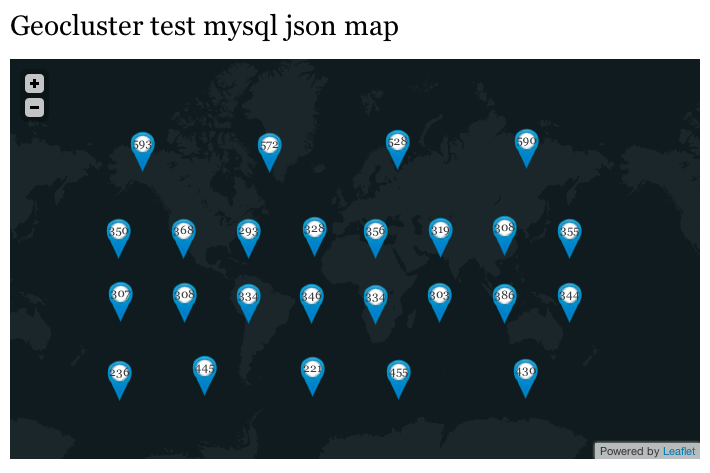
\includegraphics[width=1\textwidth]{figures/map_clustered.png}
    \caption{Geocluster visualization: a Leaflet map containing clustered markers.}
    \label{fig:map-clustered}
  \end{center}
\end{figure}

\begin{figure}[h]
  \begin{center}
    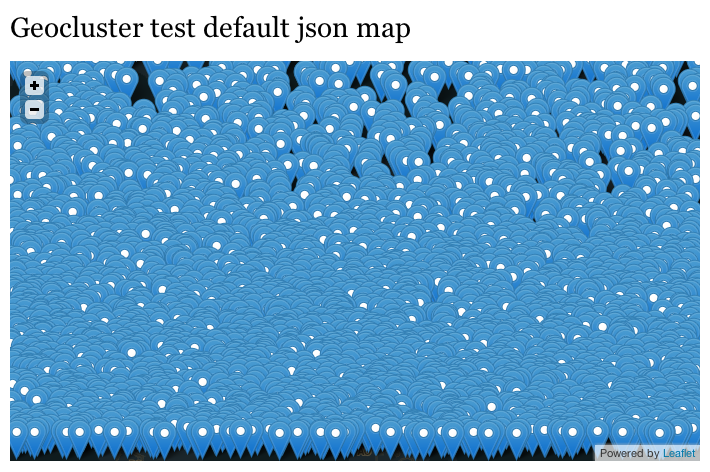
\includegraphics[width=1\textwidth]{figures/map_unclustered.png}
    \caption{Unclustered Leaflet map.}
    \label{fig:map-unclustered}
  \end{center}
\end{figure}


The Bounding Box related logic for Leaflet originally has been developed as a part of the Geocluster module. During the development process, this part of Geocluster was generalized and published as the independent Leaflet GeoJSON module\footnote{\url{http://drupal.org/project/leaflet_geojson}}. The visualization component of Geocluster therefore integrates with Leaflet GeoJSON and extends the JavaScript implementation of the Bounding Box strategy to integrate custom markers and cluster interaction. The cluster visualization is based on a code snippet for numbered markers on github\footnote{\url{https://gist.github.com/comp615/2288108}}.



%
% use cases
%

\chapter{Use cases}
\label{chapter:use-cases}

\section{Demo Use Cases}
\label{chapter:use-case-demo}

A set of demonstration use cases has been created in order to test and evaluate the Geocluster implementation described in chapter \ref{chapter:architecture-implementation}. The set consists of one non-clustering map and 3 maps based on the different clustering algorithms. The demo use cases were configured using various Drupal modules and exported into code using the Features module\footnote{\url{http://drupal.org/project/features}}.

\begin{itemize}

\item \textbf{Geocluster Demo} show cases maps based on the two clustering algorithms provided by Geocluster module: PHP-based clustering and MySQL-based clustering and an additional map that doesn't use clustering at all. The article content type of a standard Drupal installation is extended by a Geofield-based place field for storing locations. For each map, a separate View is configured to provide a GeoJSON feed. A Leaflet map is then added on top of the feed by using the Leaflet GeoJSON module. Figure \ref{fig:geocluster-demo-site} illustrates a screenshot of a Geocluster Demo installation.

\item \textbf{Geocluster Demo Solr} adds a show case of the Solr-based clustering algorithm. It provides a setup based on Views GeoJSON and Leaflet GeoJSON similar to the Geocluster Demo feature. In addition, a Search API Server and Index configuration is added for indexing and querying the data using Apache Solr.  

\item \textbf{Geocluster Demo Content} is a sub-module that automatically imports a set of demo content for testing the Geocluster Demo and Geocluster Demo Solr features.

\end{itemize}

\begin{figure}[h]
  \begin{center}
    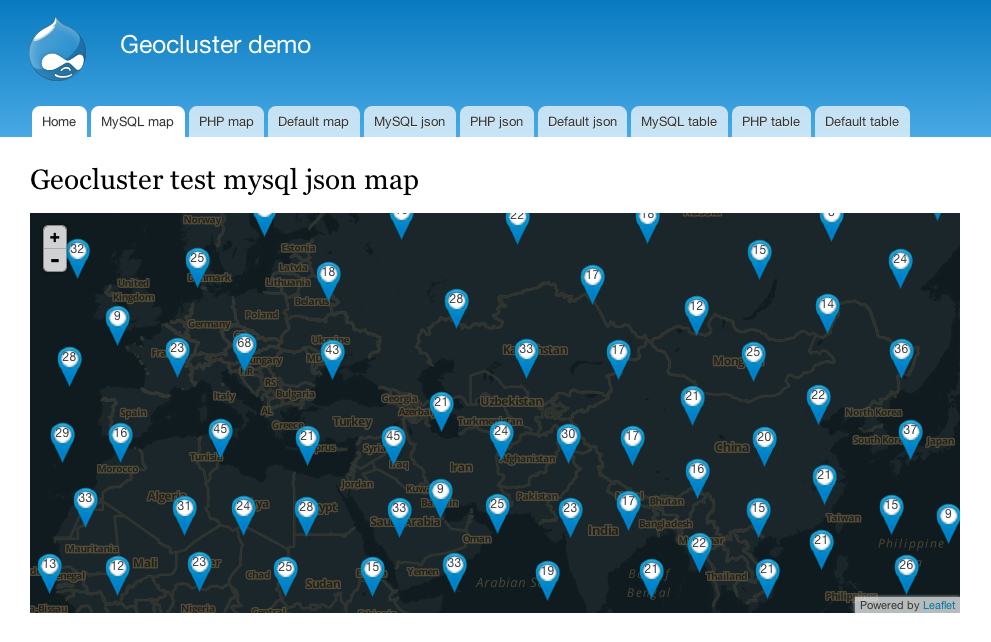
\includegraphics[width=1\textwidth]{figures/geocluster_demo_site.png}
    \caption{Screenshot of a Geocluster Demo installation. The active tab shows a map that uses MySQL-based clustering.}
    \label{fig:geocluster-demo-site}
  \end{center}
\end{figure}

\section{GeoRecruiter}
\label{chapter:use-case-georecruiter}

A practical use case for server-side geo clustering has been implemented for the Recruiter job board solution which has been introduced in chapter \ref{chapter:objective-use-cases}. It supports spatial search capabilities of the Recruiter distribution by visualizing a large amount of job offers on e-recruitment websites. GeoRecruiter allows to visualize several thousands of available jobs on an interactive map for large-scale e-recruitment websites. The Geocluster Solr module has been designed and used to provide the clustering capabilities needed by GeoRecruiter. The Solr-based aggregation integrates well with the architecture of the Recruiter distribution and is designed for scalability up to 1,000,000 indexed jobs as evaluated in chapter \ref{chapter:performance}. The prototype being discussed in the following chapter has been developed based on a copy of the Drupaljobs website\footnote{\url{http://drupaljobs.epiqo.com}}.

Drupaljobs is provided by epiqo as a show case for the Recruiter distribution. Its base features allow to create and search for job offers by companies as well as resumes of registered applicants on the e-recruitment platform. Figure \ref{fig:recruiter-job-search} depicts a screenshot of the heart of a Recruiter installation: the job search. The numbers on the figure indicate the main parts of such a page:

\begin{enumerate}

\item A \textbf{search bar (1)} above the content region.
\item \textbf{Facetted filters (2)} in the left sidebar.
\item The \textbf{search results (3)} as job teasers matching the search and filters.

\end{enumerate}

For scalability reasons, the job search functionality of Recruiter is based on Apache Solr using the Search API module which have been introduced in chapter \ref{chapter:data-storage}. The concept of using facetted filters, allows the site visitor to narrow down the result set by applying filters based on properties of the result set. The screenshot from figure \ref{fig:recruiter-job-search} displays filter facets based on \textit{organization}, \textit{fields of study} and \textit{occupational fields}. Every filter item indicates the number of results to be expected when using this particular filter. 

\begin{figure}[h]
  \begin{center}
    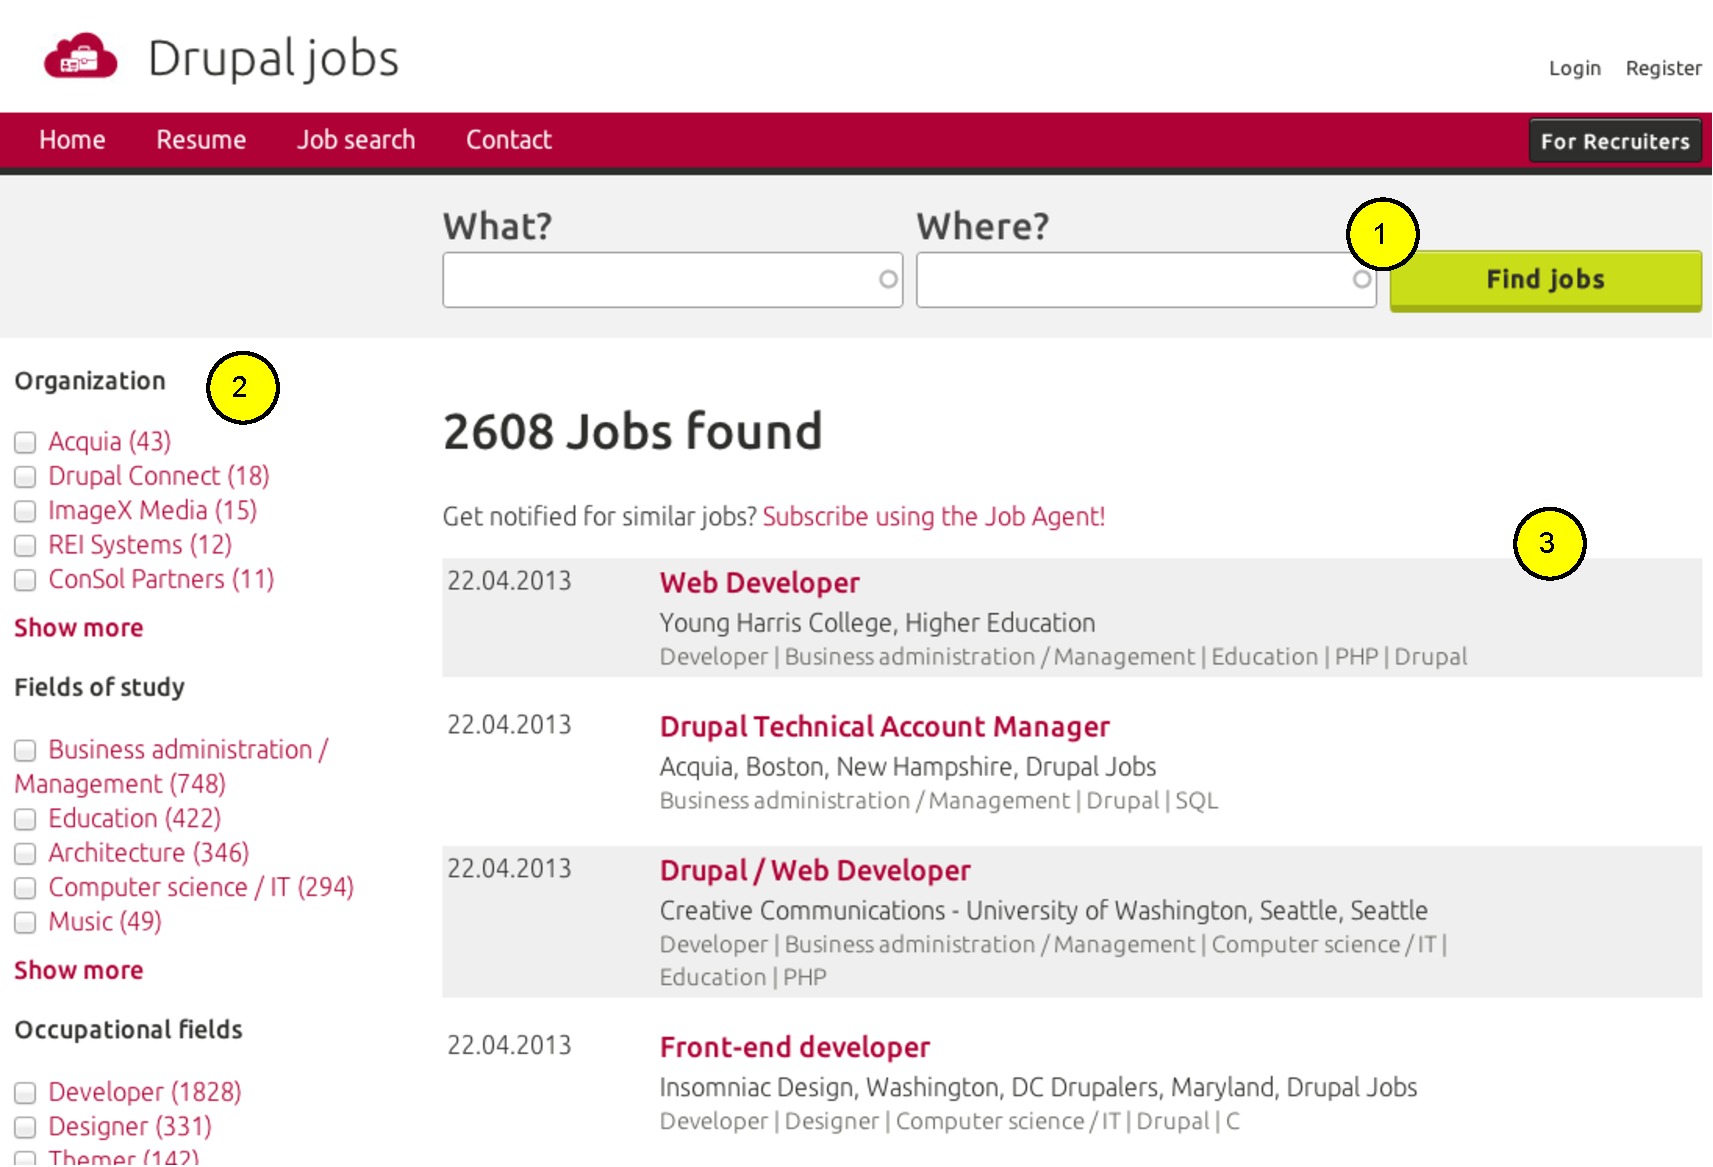
\includegraphics[width=1\textwidth]{figures/recruiter_job_search.pdf}
    \caption{Screenshot of a job search on Drupaljobs including indicators: (1) search bar, (2) facetted filters and (3) search results.}
    \label{fig:recruiter-job-search}
  \end{center}
\end{figure}

The GeoRecruiter use case consists of several geo-related additions to the Recruiter distribution. As previously stated, the customizations have been prototyped using a Drupaljobs test installation.

\begin{itemize}

\item \textbf{Add geospatial data}: The data model for posting job offers of the Recruiter distribution has been extended to support the annotation of a geospatial location as the \textit{place} property. In particular, a Geofield was added to the job node content types.

\item \textbf{Import test data}: Two sets of real-world geospatial test data have been prepared for the Drupaljobs test site. A set of 10,000 world-wide cities was created based on a dataset from GeoNames.org\footnote{\url{http://download.geonames.org/export/dump/cities1000.zip}}. Another set of 100,000 of U.S.-specific landmarks is based on a dataset from the U.S. Board on Geographic Names\footnote{\url{http://geonames.usgs.gov/docs/stategaz/NationalFile_20130404.zip}}. The kind of data isn't necessarily related to but will be mapped to job offers. This approach was taken due to the lack of a geospatially annotated datasets of job offers being available for testing purposes. Next, the test data was cleaned from errors and imported into the adapted Drupaljobs test installation. The import process was facilitated by using the Feeds module\footnote{\url{http://drupal.org/project/feeds}} which allows to import data into a Drupal site from external data sources like RSS feeds or in this particular case: CSV files.

\item \textbf{Configure Geocluster Solr}: The server-side clustering component explained in \ref{chapter:architecture-implementation} has been installed on the Drupaljobs test instance. The job search has been configured for clustering based on Apache Solr and Search API. Finally, a map visualizes the clustered job search results using Views GeoJSON and Leaflet. In order to enhance the representation of clusters and to experiment with interaction, the CSS styles of client-side clustering library Leaflet.markercluster have been adapted and extended with additional colors for large clusters.

\item \textbf{Compare with client-side clustering}: In order to measure the effectiveness of the server-side clustering approach, a client-side clustering solution has been implemented for Drupaljobs as well. The client-side clustered map is based on a blog post by Ian Whitcomb of LevelTen~\cite{blog:leaflet-made-to-order}. For querying such a large dataset, he recommends circumnavigating the Views module and directly querying the database. The client-side clustering and visualization is again realized by the Leaflet.markercluster.

\end{itemize}

The resulting prototype allowed to experiment with the server-side clustering solution in a realistic environment, draw conclusions on effectiveness of clustering algorithm and the visualization component being used. A visualization of a map within the Drupaljobs test installation is provided in figure \ref{fig:drupaljobs-geocluster-solr}.

\begin{figure}[h]
  \begin{center}
    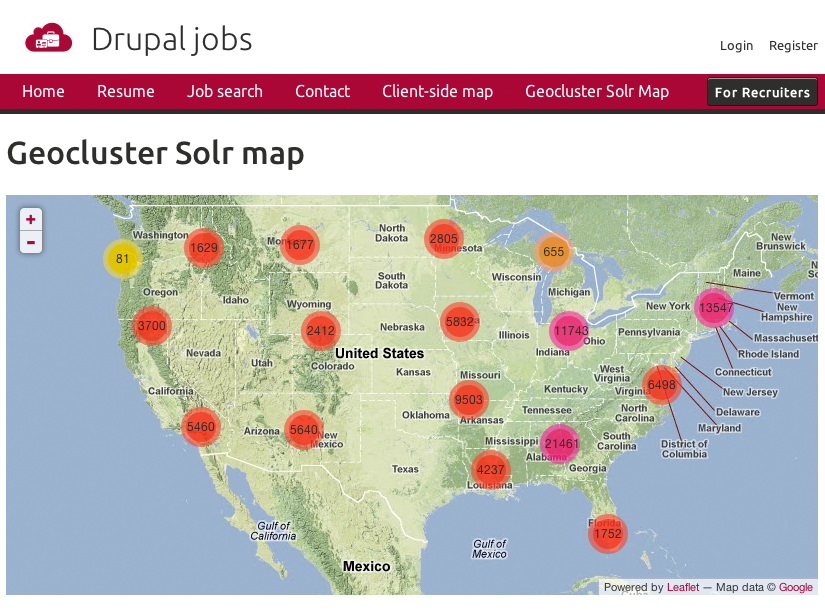
\includegraphics[width=1\textwidth]{figures/drupaljobs_geocluster_solr.png}
    \caption{Screenshot of map that visualized job search results on a map using Solr-based clustering on a Drupaljobs test installation.}
    \label{fig:drupaljobs-geocluster-solr}
  \end{center}
\end{figure}


Besides the clustering functionality, GeoRecruiter will support location-based search. This allows the user to search for jobs within the surroundings of a desired region by applying a proximity filter. The Search API Location module is currently being refactored\footnote{\url{http://drupal.org/node/1798168}} in order to provide a solid foundation for such spatial queries using Solr and the Search API module suite.


\section{Further evaluation}

The second objective on integration and extensibility defined in chapter \ref{chapter:objective-integration} has been fulfilled by the Geocluster module as it integrates with Views, Views GeoJSON and other Drupal mapping modules. In addition, the implementation of the clustering algorithm can be extended using plugins as explained in chapter \ref{chapter:impl-alg}. Geocluster was also released under the GPL license as required by objective \ref{chapter:open-source}. With regards to objective \ref{chapter:objective-use-cases}, a demo use case has been implemented that show cases all the functionality needed. The actual GeoRecruiter use case hasn't been implemented, but as stated in \ref{chapter:use-case-georecruiter}, the groundwork has been established in order to do so. Finally, main usability concerns have been realized with the Geocluster Visualization component.

While most objectives have been reached, there are still many parts of the Geocluster implementation that can be improved upon:

\begin{itemize}

\item \textbf{Cluster sizes}: The current implementation doesn't respect the size of a cluster. As naturally, a cluster with more items can be visualized larger than smaller clusters, the algorithm could be improved for growing clusters by their size. The bigger size of a cluster would therefore reduce the distance to its neighbor clusters, potentially merging additional neighbors into it. Andrew Betts describes a similar approach under the term \textit{``Grid based viral growth argorithm''}~\cite{web:clustering-google}.

\item \textbf{Cluster centers}: While the PHP- and MySQL-based algorithm provide means of calculating a centroid as the center of a cluster, the Solr-based clustering algorithm is limited in this regards. Solr doesn't seem to provide the same functionality to calculate the mean value for a field using the grouping function, as the MySQL-based algorithm leverages the $AVG$ function for latitude and longitude. Potentially, the stats component\footnote{\url{http://wiki.apache.org/solr/StatsComponent}} could be used for calculating the centroid of cluster items within the Solr-based algorithm.

\item \textbf{Processing clustered results}: The way that the Drupal mapping stack integrates with the Views module isn't designed for processing clustered results. The current implementation of Geocluster performs various workarounds in order to inject clustered results into the process. Especially for the Solr-based implementation this leads to code-duplication because in the standard case results are processed as arrays while in the other case, results need to be PHP objects. If possible, a cleaner way of integrating clustering with the related modules is desirable.   

\item \textbf{Improve client-side handling and visualization}: The current implementation for visualizing clustered results is very basic: as the screenshot of the Geocluster Demo installation in figure \ref{fig:geocluster-demo-site} shows, cluster sizes are only indicated by printing the number within markers. 

 A relative sizing of cluster items according to their clusters is needed and should also be supported by the algorithm as stated before. In addition, it would be good to have be a clean way to configre the how data for clustered results should be displayed and integrate it with how non-clustered data is represented. For low zoom levels, the roundtrip to the server for fetching a separate clustered result on every bounding box change can be an overhead. Christopher Calid\footnote{\url{http://drupal.org/user/210499}} proposed a way of ``Progressively enhance server-side with client-side clustering''\footnote{\url{http://drupal.org/node/1914704}}. The intention is to transition from server-side clustering higher zoom levels to client-side clustering for lower zoom levels.

\end{itemize}








\newpage

 \appendix
% \chapter{Acronyms}

\begin{acronym}
\acro{AJAX}{Asynchronous JavaScript + XML}
\acro{API}{Application Programming Interface}
\acro{CMS}{Content Management System}
\acro{GNU}{GNU's Not Unix}
\acro{HTML}{HyperText Markup Language}
\acro{HTTP}{HyperText Transfer Protocol}
\acro{IDE}{Integrated Development Environment}
\acro{IT}{Information Technology}
\acro{JSON}{JavaScript Object Notation}
\acro{OASIS}{Organization for the Advancement of Structured Information
Standards}
\acro{REST}{Representational State Transfer}
\acro{RSS}{Really Simple Syndication}
\acro{UDDI}{Universal Description, Discovery and Integration}
\acro{UI}{User Interface}
\acro{URI}{Uniform Resource Identifier}
\acro{URL}{Uniform Resource Locator}
\acro{W3C}{World Wide Web Consortium}
\end{acronym}

 \chapter{Index}
\listoffigures
\listoftables
% \lstlistoflistings

%%%%%%%%%%%%%%%%%%%%%%%%%%%%%%%%%%%%%%%%
% PUT APPENDIX, BIBLIOGRAPHY, ... HERE %
%%%%%%%%%%%%%%%%%%%%%%%%%%%%%%%%%%%%%%%%

\bibliographystyle{alpha}
%\bibliographystyle{alpha}
\bibliography{bib/references}

\end{document}

%%% Local Variables:
%%% TeX-PDF-mode: t
%%% TeX-debug-bad-boxes: t
%%% TeX-master: t
%%% TeX-parse-self: t
%%% TeX-auto-save: t
%%% reftex-plug-into-AUCTeX: t
%%% End: